\section{Complications}

[Very drafty.  These are just notes.]

Complications:
\begin{itemize}
\item Dependency: preconditions
\item TC1: Track local state
\item Release/Acquire: $\mathsf{Q}$
\item Coherence respects program order: $\mathsf{Q}_{x}$
\item Drop read-read coherence: $\mathsf{QW}_{x}$ (Required for CSE without
  alias analysis over read only code, not required by hardware)
\item Address calculation...
\item No read-read dependency (for arm): $\mathsf{RW}$/$\mathsf{RO}$ (control
  dependencies into reads as in MP with release on right and control
  dependency on left)
\item Downgrading acquires/Anton example: ${\downarrow} x$
\end{itemize}
Require indexing by event:
\begin{itemize}
\item IF closure/case analysis: $\psi_e$
\item Redundant read elimination/TC2, to get determinism of value per event
\end{itemize}



\subsection{Triangle Races}


\begin{gather*}
  \PW{x}{1}\SEMI
  \PW[\mRA]{y}{1}\SEMI
  \PR[\mRA]{x}{r}
  \PAR
  \IF{\PR[\mRA]{y}{}}\THEN \PW[\mRA]{x}{2}\FI
  \\
  \hbox{\begin{tikzinline}[node distance=1.5em]
      \event{a1}{\DW{x}{1}}{}
      \event{a2}{\DW[\mRA]{y}{1}}{right=of a1}
      \event{a3}{\DR[\mRA]{x}{1}}{right=of a2}
      \event{b1}{\DR[\mRA]{y}{1}}{right=3em of a3}
      \event{b2}{\DW[\mRA]{x}{2}}{right=of b1}
      \sync{a1}{a2}
      \rf[out=20,in=160]{a1}{a3}
      \rf[out=20,in=160]{a2}{b1}
      \sync{b1}{b2}
    \end{tikzinline}}
  \\
  \hbox{\begin{tikzinline}[node distance=1.5em]
      \event{a1}{\DW{x}{1}}{}
      \event{a2}{\DW[\mRA]{y}{1}}{right=of a1}
      \event{a3}{\DR[\mRA]{x}{2}}{right=of a2}
      \event{b1}{\DR[\mRA]{y}{1}}{right=3em of a3}
      \event{b2}{\DW[\mRA]{x}{2}}{right=of b1}
      \sync{a1}{a2}
      \rf[out=20,in=160]{a2}{b1}
      \rf[out=160,in=20]{b2}{a3}
      \sync{b1}{b2}
    \end{tikzinline}}
\end{gather*}
Bug is in \citep[Lemma A.4]{DBLP:conf/ppopp/DongolJR19}.  It assumes that
$\DRP[\mRA]{x}{1}$ and $\DWP[\mRA]{x}{2}$ are racing in the first execution
because they are not ordered by happens-before.  But this is false since
neither is plain.



\subsection{TC2}

\begin{gather*}
  \taglabel{TC2}
  \PR{x}{r}\SEMI
  \PR{x}{s}\SEMI
  \IF{r{=}s}\THEN \PW{y}{1}\FI
  \PAR
  x\GETS y
  \\
  \hbox{\begin{tikzinline}[node distance=1.5em]
  \event{a1}{\DR{x}{1}}{}
  \event{a2}{\DR{x}{1}}{right=of a1}
  \event{a3}{\DW{y}{1}}{right=of a2}
  % \po{a2}{a3}
  % \po[out=-20,in=-160]{a1}{a3}
  \event{b1}{\DR{y}{1}}{right=3em of a3}
  \event{b2}{\DW{x}{1}}{right=of b1}
  \rf{a3}{b1}
  \po{b1}{b2}
  \rf[out=169,in=11]{b2}{a2}
  \rf[out=169,in=11]{b2}{a1}
    \end{tikzinline}}
\end{gather*}
Precondition of $\DWP{y}{1}$ is $(r{=}s)$ in
\begin{math}
  \sem{\IF{r{=}s}\THEN y\GETS 1\FI}.
\end{math}
Predicate transformers for $\emptyset$ in $\sem{\PR{x}{r}}$ and $\sem{\PR{x}{s}}$ are
\begin{align*}
  \PREDP{(r{=}1 \lor r{=}x)\limplies\aForm[r/x]},
  \\
  \PREDP{(s{=}1 \lor s{=}x)\limplies\aForm[s/x]}.
\end{align*}
Combining the transformers, we have
\begin{displaymath}
  \PREDP{(r{=}1 \lor r{=}x)\limplies(s{=}1 \lor s{=}r)\limplies\aForm[s/x]}.
\end{displaymath}
Applying this to $(r{=}s)$, we have
\begin{displaymath}
  \PREDP{(r{=}1 \lor r{=}x)\limplies (s{=}1 \lor s{=}r)\limplies (r{=}s)},
\end{displaymath}
which is not a tautology.

Same problem occurs oopsla, where we have:
\begin{align*}
  \PREDP{\aForm[v/x,r] \land \aForm[x/r]},
  \\
  \PREDP{\aForm[v/x,s] \land \aForm[x/s]}.
\end{align*}
Combining the transformers, we have
\begin{displaymath}
  \PREDP{\aForm[v/x,r,s] \land \aForm [v/x,r][x/s] \land \aForm[x/r][v/x,s] \land \aForm[x/r,s]}.
\end{displaymath}
Applying this to $(r{=}s)$, we have
\begin{displaymath}
  \PREDP{v{=}v \land v{=}x \land x{=}v \land x{=}x},
\end{displaymath}
which is not a tautology.

The semantics here allows this by coalescing:
\begin{gather*}
  r\GETS x\SEMI
  s\GETS x\SEMI
  \IF{r{=}s}\THEN y\GETS 1\FI
  \PAR
  x\GETS y
  \\
  \hbox{\begin{tikzinline}[node distance=1.5em]
      \event{a1}{\DR{x}{1}}{}
      \event{a3}{\DW{y}{1}}{right=of a1}
      \event{b1}{\DR{y}{1}}{right=3em of a3}
      \event{b2}{\DW{x}{1}}{right=of b1}
      \rf{a3}{b1}
      \po{b1}{b2}
      \rf[out=169,in=11]{b2}{a1}
    \end{tikzinline}}
\end{gather*}

\subsection{Coherence}
Can be encoded in independency, or logic.

\subsection{Release Acquire}
Can be encoded in independency, or logic, but logic is more flexible, and we
need that for \armeight.


\subsection{Agda}

\begin{figure*}
  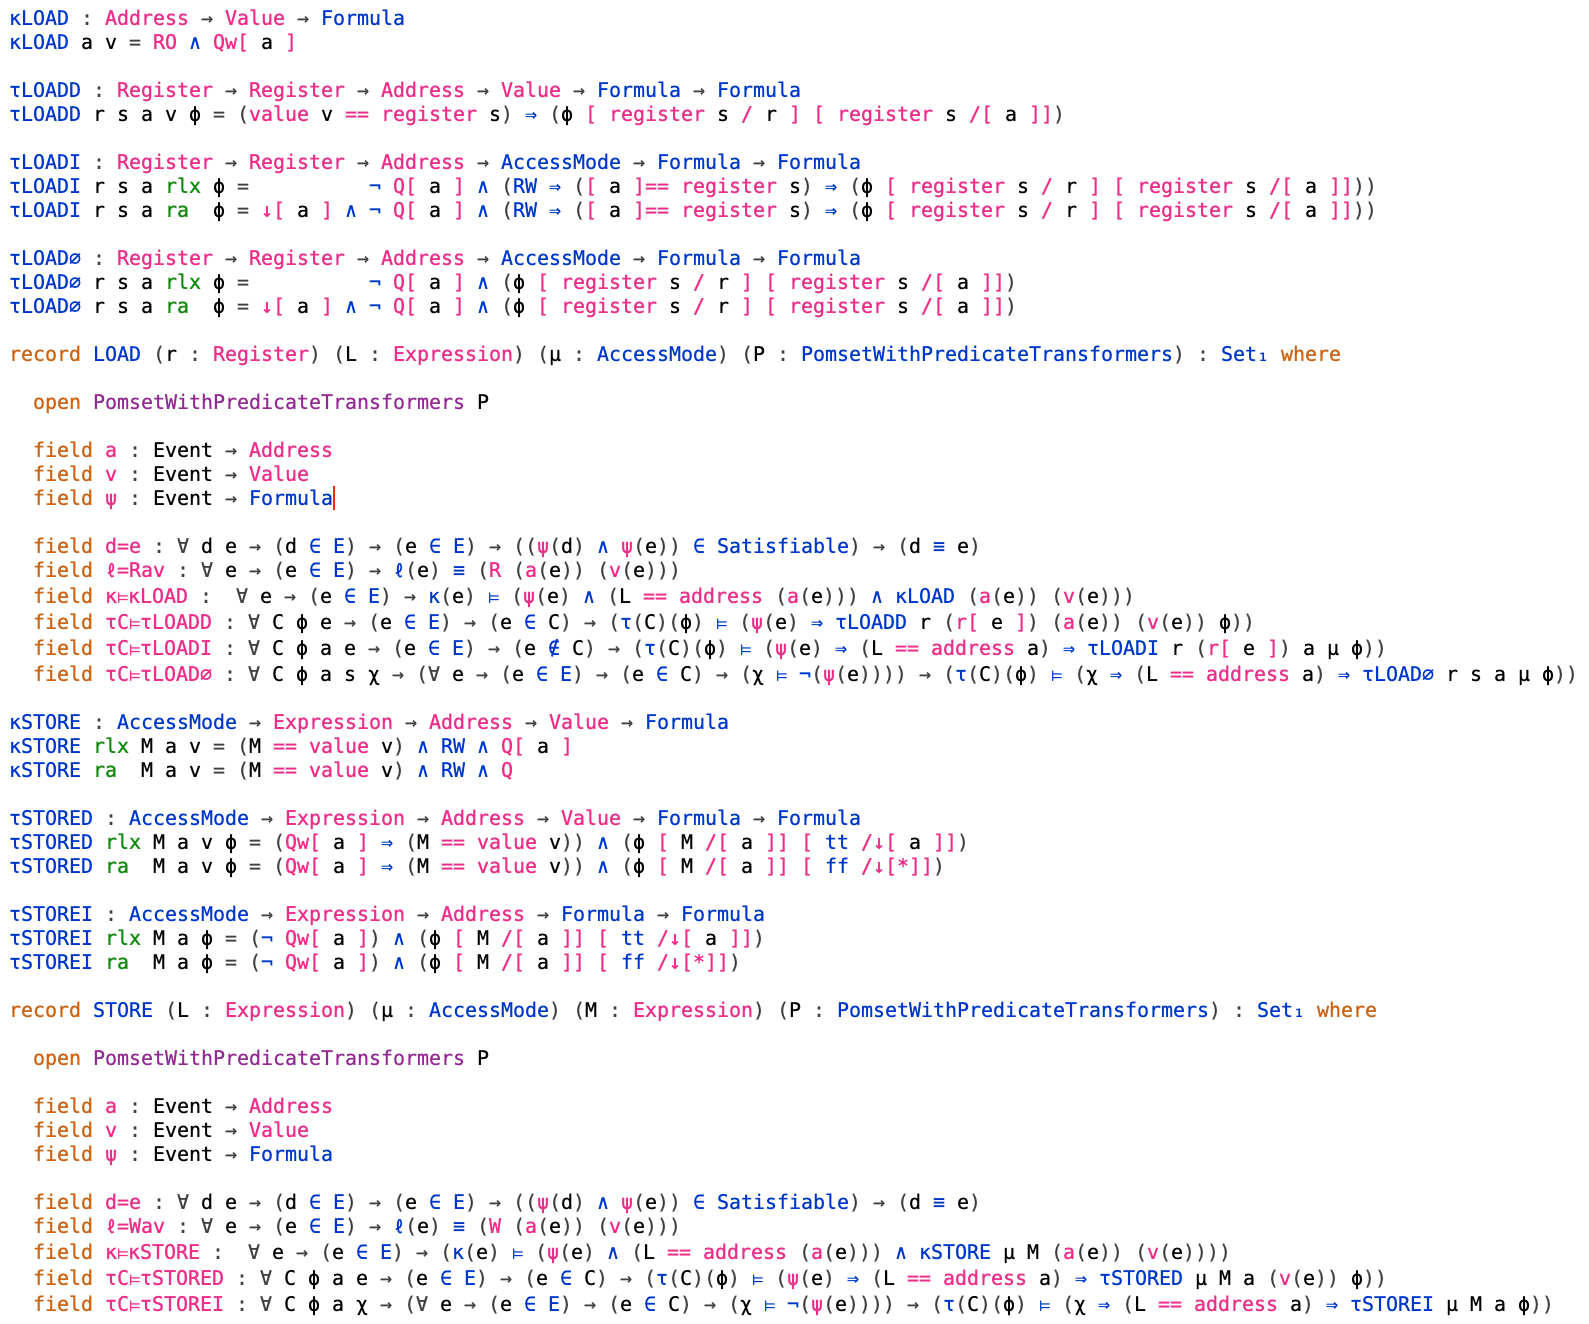
\includegraphics[width=\textwidth]{agda.png}
\end{figure*}
